\documentclass[aspectratio=1610,handout]{beamer}
\usepackage{hyperref}
\usepackage[T1]{fontenc}
\usefonttheme[onlymath]{serif}

% other packages
\usepackage{latexsym,amsmath,xcolor,multicol,booktabs,calligra}
\usepackage{graphicx,pstricks,listings,stackengine}
\usepackage{
	amsfonts,
	amssymb,
	bm,
	mathrsfs,
	xparse,
	%esint,
	physics2,
	pgfplots,
	mathrsfs,
	perpage,
	ulem,
	amsthm,
	geometry,
	upgreek,
	%mathptmx,
	%txfonts,
	lmodern,
	gbt7714,
	subcaption,
	booktabs,
	cases,
	tcolorbox,
	tabularx,
	longtable,
    xcolor,
    fixdif,
    derivative,
    subcaption
}

\pgfplotsset{compat=1.15}
\usetikzlibrary{arrows,arrows.meta}
\definecolor{uuuuuu}{rgb}{0.26666666666666666,0.26666666666666666,0.26666666666666666}

\usephysicsmodule{ab,ab.legacy,diagmat}

\makeatletter
\newcommand\vb{\@ifstar\boldsymbol\mathbf}
\newcommand\va[1]{\@ifstar{\vec{#1}}{\vec{\mathrm{#1}}}}
\newcommand\vu[1]{%
\@ifstar{\hat{\boldsymbol{#1}}}{\hat{\mathbf{#1}}}}
\makeatother

\newcommand\bmqty[1]{\begin{bmatrix}#1\end{bmatrix}}
\newcommand\pmqty[1]{\begin{pmatrix}#1\end{pmatrix}}

\usetikzlibrary{angles,quotes,patterns,decorations.markings,arrows.meta}

\hypersetup{bookmarks=true,bookmarksopen=false,pdfstartview=FitV}

\DeclareSymbolFont{EulerExtension}{U}{euex}{m}{n}
\DeclareMathSymbol{\euintop}{\mathop} {EulerExtension}{"52}
\DeclareMathSymbol{\euointop}{\mathop} {EulerExtension}{"48}
\let\intop\euintop
\let\ointop\euointop

\newcommand{\im}{\mathrm{i}}
\newcommand{\ex}[1]{\mathrm{e}^{#1}}
\newcommand{\avg}[1]{\left\langle{#1}\right\rangle}
\DeclareMathOperator{\res}{res}
\newcommand{\dotv}[1]{\dot{\vb*{#1}}}
\newcommand{\alarm}[1]{\textcolor{red}{#1}}

\author{Your Name}
\title[WHU Beamer Template]{\bfseries WHU Beamer Template\\ Demo \& Usage Guide}
\subtitle{}
\institute{Your Institution}
\date{\today}
\usepackage{whu}

\hypersetup{pdftitle={WHU Beamer Template Demo},pdfauthor={}}

% defs
\def\cmd#1{\texttt{\color{red}\footnotesize $\backslash$#1}}
\def\env#1{\texttt{\color{blue}\footnotesize #1}}
\definecolor{deepblue}{rgb}{0,0,0.5}
\definecolor{deepred}{rgb}{0.6,0,0}
\definecolor{deepgreen}{rgb}{0,0.5,0}
\definecolor{halfgray}{gray}{0.55}

\lstset{
    basicstyle=\ttfamily\small,
    keywordstyle=\bfseries\color{deepblue},
    emphstyle=\ttfamily\color{deepred},    % Custom highlighting style
    stringstyle=\color{deepgreen},
    numbers=left,
    numberstyle=\small\color{halfgray},
    rulesepcolor=\color{red!20!green!20!blue!20},
    frame=shadowbox,
}

\setbeamertemplate{background}{
\includegraphics[width=\paperwidth,height=\paperheight]{images/background_1610.png}}
% bg-image: use png, pdf, or jpg format (eps not supported for background)

\begin{document}

\begin{frame}
    \titlepage
    \begin{figure}[htpb]
        \begin{center}
            
\includegraphics[width=0.13\linewidth]{pic/whulogo+.png}
        \end{center}
    \end{figure}
\end{frame}

\begin{frame}
    \frametitle{Outline}
    \tableofcontents[sectionstyle=show,subsectionstyle=show/shaded/hide,subsubsectionstyle=show/shaded/hide]
\end{frame}

\section{Getting Started}

\begin{frame}
    \frametitle{What is This Template?}
    \begin{itemize}
        \item A \textbf{WHU (Wuhan University)} themed Beamer template for academic presentations.
        \item Modified from \href{https://github.com/xinchen13/WHU-Beamer-Theme}{\texttt{xinchen13/WHU-Beamer-Theme}}.
        \item Background images from \href{https://github.com/hrtan99/WHU-Beamer}{\texttt{hrtan99/WHU-Beamer}}.
        \item Color scheme uses the official WHU ``Luojia Green'' (\texttt{whucolor}).
        \item Supports both \textbf{16:10} and \textbf{16:9} aspect ratios.
        \item A \textbf{Chinese version} (\texttt{Slide-zh.tex}) is also included, with \texttt{ctex} support.
    \end{itemize}
\end{frame}

\begin{frame}[fragile]
    \frametitle{Quick Start}
    \begin{enumerate}
        \item Change the metadata in the preamble:
        \begin{lstlisting}[language=TeX]
\author{Your Name}
\title{Your Presentation Title}
\institute{Your Institution}
\date{\today}
        \end{lstlisting}
        \item Add your content in \verb|\begin{document} ... \end{document}|.
        \item Compile with \textbf{pdflatex} (English) or \textbf{xelatex} (Chinese):
        \begin{lstlisting}[language=bash]
pdflatex Slide.tex
bibtex Slide
pdflatex Slide.tex
pdflatex Slide.tex
        \end{lstlisting}
    \end{enumerate}
\end{frame}

\section{Template Features}

\begin{frame}
    \frametitle{Basic Blocks}
    \begin{block}{Standard Block}
        This is a standard \texttt{block} environment. Use it for general content.
    \end{block}
    \pause
    \begin{alertblock}{Alert Block}
        This is an \texttt{alertblock}. Use it to highlight important information.
    \end{alertblock}
    \pause
    \begin{exampleblock}{Example Block}
        This is an \texttt{exampleblock}. Use it for examples and illustrations.
    \end{exampleblock}
\end{frame}

\begin{frame}
    \frametitle{Columns Layout}
    \begin{columns}[T]
        \begin{column}{0.5\textwidth}
            \begin{block}{Left Column}
                \begin{itemize}
                    \item Item 1
                    \item Item 2
                    \item Item 3
                \end{itemize}
            \end{block}
        \end{column}
        \begin{column}{0.5\textwidth}
            \begin{block}{Right Column}
                \begin{enumerate}
                    \item First point
                    \item Second point
                    \item Third point
                \end{enumerate}
            \end{block}
        \end{column}
    \end{columns}
\end{frame}

\begin{frame}
    \frametitle{Figures and Images}
    \begin{columns}[T]
        \begin{column}{0.5\textwidth}
            \begin{itemize}
                \item Use \cmd{includegraphics} to insert figures.
                \item Supported formats: \texttt{png}, \texttt{pdf}, \texttt{jpg}.
                \item Place your images in the \texttt{images/} or \texttt{pic/} folders.
            \end{itemize}
        \end{column}
        \begin{column}{0.5\textwidth}
            \centering
            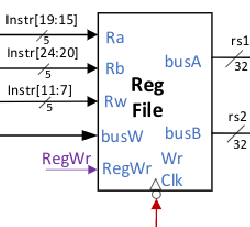
\includegraphics[width=0.8\linewidth]{pic/demo.png}
            \captionof{figure}{Demo figure (\texttt{pic/demo.png})}
        \end{column}
    \end{columns}
\end{frame}

\begin{frame}
    \frametitle{Mathematical Equations}
    The template includes commonly used math commands:
    \begin{itemize}
        \item \cmd{vb\{x\}} for bold vectors: $\vb{x}$, $\vb*{x}$
        \item \cmd{va\{x\}} for arrow vectors: $\va{x}$, $\va*{x}$
        \item \cmd{vu\{x\}} for unit vectors: $\vu{x}$, $\vu*{x}$
        \item \cmd{bmqty}, \cmd{pmqty} for matrices: $\bmqty{a & b \\ c & d}$
        \item \cmd{im} for imaginary unit, \cmd{ex\{x\}} for exponential
        \item \cmd{avg\{x\}} for expectation values: $\avg{x}$
    \end{itemize}
    Example equation:
    \[
        \odv[2]{\mathcal{I}_{ik}}{t} = 2\mathcal{T}_{ik} - 2\mathcal{M}_{ik} + \mathcal{E}_{ik} + \mathcal{P}_{ik} + \delta_{ik}\mathcal{M}
    \]
\end{frame}

\section{Customization}

\begin{frame}[fragile]
    \frametitle{Changing Background Images}
    \begin{itemize}
        \item The background is set in the preamble:
        \begin{lstlisting}[language=TeX]
\setbeamertemplate{background}{
  
\includegraphics[width=\paperwidth,
                    height=\paperheight]
  {images/background_1610.png}
}
        \end{lstlisting}
        \item Two aspect ratios are provided:
        \begin{itemize}
            \item \texttt{images/background\_1610.png} — for 16:10
            \item \texttt{images/background\_169.png} — for 16:9
        \end{itemize}
        \item Cover backgrounds are also available:
        \begin{itemize}
            \item \texttt{images/background\_cover\_1610.png}
            \item \texttt{images/background\_cover\_169.png}
        \end{itemize}
    \end{itemize}
\end{frame}

\begin{frame}[fragile]
    \frametitle{Switching Aspect Ratio}
    \begin{itemize}
        \item Change the document class option:
        \begin{lstlisting}[language=TeX]
\documentclass[aspectratio=1610]{beamer}  % 16:10
\documentclass[aspectratio=169]{beamer}   % 16:9
        \end{lstlisting}
        \item Remember to update the background image path accordingly!
        \item The \texttt{handout} option can be removed for presentation mode (shows overlays).
    \end{itemize}
\end{frame}

\section{Credits \& License}

\begin{frame}
    \frametitle{Acknowledgments}
    \begin{block}{Upstream Projects}
        \begin{itemize}
            \item This template is modified from\\
            \href{https://github.com/xinchen13/WHU-Beamer-Theme}{\texttt{xinchen13/WHU-Beamer-Theme}}
            \item Background images are from\\
            \href{https://github.com/hrtan99/WHU-Beamer}{\texttt{hrtan99/WHU-Beamer}}
        \end{itemize}
    \end{block}
    \pause
    \begin{alertblock}{License}
        This project is licensed under the \textbf{LaTeX Project Public License v1.3c (LPPL-1.3c)}, consistent with the upstream repositories. See the \texttt{LICENSE} file for details.
    \end{alertblock}
\end{frame}

\begin{frame}[allowframebreaks]
    \frametitle{References}\small
    \nocite{*}
    \bibliography{ref}
\end{frame}

\begin{frame}
    \centering
    \Huge
    {\calligra Thanks!}

    \vspace{1cm}
    \normalsize
    \href{https://github.com/ryan-gwo/WHU-Beamer-Template}{\texttt{github.com/ryan-gwo/WHU-Beamer-Template}}
\end{frame}

\end{document}
